\documentclass[11pt,a4paper]{jreport}
%
\usepackage{amsmath,amssymb}
\usepackage{bm}
\usepackage[dvipdfmx]{graphicx}
\usepackage{ascmac}
\usepackage{tabularx}
%
%
\newcommand{\divergence}{\mathrm{div}\,}  %ダイバージェンス
\newcommand{\grad}{\mathrm{grad}\,}  %グラディエント
\newcommand{\rot}{\mathrm{rot}\,}  %ローテーション
%
\pagestyle{myheadings}
\begin{document}
%
%
\chapter*{◆やさしいPython◆}
\begin{flushright}
  2020年数理物理学研究室 村上作成
\end{flushright}
『やさしいPython』 著:高橋麻奈 をまとめてtex打ちしたもの。誤植も多いと思うが悪しからず。



\tableofcontents

\chapter{はじめの一歩}% Lesson1 %
\section{入力方法}
Atomを利用。追加パッケージは大体以下の通り。
\begin{itemize}
 \item atom-beautify
 \item atom-ide-ui
 \item atom-runner
 \item atom-terminal
 \item autocomplete-python
 \item highlight-colum
 \item linter-python-pep8
\end{itemize}
デフォルトで日本語を表示させようとすると文字化けするので、
左上のFileタブ→起動スクリプト→init.coffeeのファイルに\\
process.env.PYTHONIOENCODING = "utf-8";\\
を追加して保存→再起動させると、文字化けが無くなる。\\

AtomのAtom-runnerパッケージでは入力ができないので、他のターミナルでコンパイルするほうが良い。

\section{蛇足-Git-}
\TeX 打ちをしながら本を読んでいたら、誤って上書き保存してしまい、やる気が無くなった

\chapter{Pythonの基本}% Lesson2 %
\section{コードの内容}
\begin{shadebox}
 \#画面に出力する\\
 print("Hello World")\\
 print("Let's start Python")
\end{shadebox}
\vspace{0.2in}
\begin{screen}
 Hello World\\
 Let's start Python
\end{screen}
\vspace{0.2in}
\subsection{新しいコードを入力する}
画面に表示させることを"出力する"ともいう。出力するには、print(・・・)というコードを記述する。

\subsection{コメントを記述する}
プログラムの実行とは直接関係のない自分の言葉をメモできる。(コメント) チームでプログラムを作成するときや、自分で見直す際にわかりやすい。\\
\#の後の一文はコメントとして無視される。

\subsection{1文ずつ処理する}
Pythonでは1つの小さな処理を文(Statement)と呼ぶ。この"文"が
\begin{center}
 (原則として)先頭から順番に1文ずつ処理される
\end{center}
ことになっている。

\section{文字列と数値}
\subsection{文字列リテラル}
文字の並びを{\bf 文字列リテラル(string literal)}という。文字列は「'」または「"」でくくって記述する(どちらでも良い)\\
Pythonでは、次のように3つの「'」、「"」でくくると、改行を含めた文字列を作ることができる。

\begin{shadebox}
 \#画面に出力する\\
 print("""Hello
 World""")\\
 print('''Let's
 start
 Python''')
\end{shadebox}
\vspace{0.2in}
\begin{screen}
 Hello
 world!
 Let's
 start
 Python!
\end{screen}
\vspace{0.2in}

\subsection{数値リテラル}
数値には次のような種類がある。
\begin{itemize}

 \item {\bf 整数リテラル(integer)} 1、3、100など
 \item {\bf 浮動小数点数リテラル(floating)} 2.1、3.14、5.0など
 \item {\bf 虚数リテラル(imaginary)} 数字にjをつけたもの

\end{itemize}
数字のリテラルは「"」や「'」でくくらないことに注意

\subsection{n進数を使う}
プログラムの世界では、2進数、8進数、16進数がよく使われる。Pythonでこれらの数値を表す場合には、数値の先頭に次の表記を付けて表す。

\begin{itemize}
 \item {\bf 2進数} 数値の先頭に0bを付ける
 \item {\bf 8進数} 数値の先頭に0oを付ける
 \item {\bf 16進数} 数値の先頭に0xを付ける
\end{itemize}

\begin{shadebox}
 \#n進法\\

 print("10進数の10は10進数でいうと", 10 ,"です")\\
 print("2進数の10は10進数でいうと", 0b10 ,"です")\\
 print("8進数の10は10進数でいうと", 0o10 ,"です")\\
 print("16進数の10は10進数でいうと", 0x10 ,"です")\\
 print("16進数のFは10進数でいうと", 0xF ,"です")

\end{shadebox}
\vspace{0.2in}
\begin{screen}
 10進数の10は10進数でいうと 10 です\\
 2進数の10は10進数でいうと 2 です\\
 8進数の10は10進数でいうと 8 です\\
 16進数の10は10進数でいうと 16 です\\
 16進数のFは10進数でいうと 15 です
\end{screen}
\vspace{0.2in}

\subsection{エスケープシーケンスを使う}
文字の中には、1文字で表せない特殊な文字がある。このような文字をprint()によって出力する際には、\textbackslash との組み合わせで1文字を表す。これを{\bf エスケープシーケンス(escape sequence)}という。

\begin{table}[h]
 \begin{tabular}{|l|l|} \hline
  エスケープシーケンス          & 意味している文字               \\ \hline \hline
  \textbackslash t              & 水平タブ                       \\
  \textbackslash v              & 垂直タブ                       \\
  \textbackslash n              & 改行                           \\
  \textbackslash r              & 復帰                           \\
  \textbackslash a              & 警戒音                         \\
  \textbackslash b              & バックスペース                 \\
  \textbackslash f              & 改ページ                       \\
  \textbackslash '              & '                              \\
  \textbackslash "              & "                              \\
  \textbackslash \textbackslash & \textbackslash                 \\
  \textbackslash ○○○            & 8進数○○○の文字コードを持つ数字 \\
  \textbackslash xhh            & 16進数hhの文字コードを持つ文字 \\ \hline
 \end{tabular}

\end{table}

また、文字列の前にrまたはRをつけると、¥をエスケープシーケンスとして扱わない文字列を作成することができる。{\bf (raw文字列)}

\begin{shadebox}
 \#raw文字列\\
 print("バックスラッシュを表示:\textbackslash")\\
 print(r"バックスラッシュを表示:\textbackslash")
\end{shadebox}
\vspace{0.2in}
\begin{screen}
 バックスラッシュを表示:\\
 バックスラッシュを表示:\textbackslash
\end{screen}
\vspace{0.2in}


\chapter{変数と式}% Lesson3 %
\section{変数}
\subsection{変数の仕組み}
変数:コンピューター内部にあるいろいろな値を記録しておくための{\bf メモリ(memory)}を利用して、値を記録する仕組み。変数というハコの中に値を入れるように、特定の値を入れることができる。

\subsection{変数の名前を決める}
\begin{itemize}

 \item 英字・数字・アンダースコア(\_)のいずれかを用いる。
 \item 数字では始められない
 \item 大文字と小文字は区別する
 \item コード上意味を持つ言葉を使うことができない

\end{itemize}

このような規則に従う名前を、{\bf 識別子(identifier)}と呼ぶ。

\subsection{変数に値を代入する}
変数に特定の値を記憶させることを、{\bf 値を代入する}という。「=」という記号は、値を記憶させる機能を持っている。Pythonの変数は、初めて値を代入したときにメモリ上に作成される。

\subsection{変数を利用する}
変数をprintすると、変数の中に入っている値が出力される。
\begin{shadebox}
 \#変数への代入と利用\\
 \#変数名 = 式\\
 sale = 10\\
 print("売り上げは", sale, "万円です。")
\end{shadebox}
\vspace{0.2in}
\begin{screen}
 売り上げは 10 万円です。
\end{screen}
\vspace{0.2in}

\subsection{変数の値を変更する}
変数の値は上書きすることができる。

\subsection{その他の型を格納する}
変数には数字の他、様々な値を格納することができる。

\begin{itembox}[htbp]{型}
 変数に格納できる値の種類を{\bf 型(type)}と呼ぶ。
 Pythonの主な型には、下表のようなものがある。

\end{itembox}


\begin{table}[htbp]
 \begin{center}
  \begin{tabular}{|ll|} \hline
   数値         & 整数(int)            \\
                & 真偽値(bool)         \\
                & 浮動小数点数(float)  \\
                & 複素数(complex)      \\ \hline
   シーケンス   & リスト(list)         \\
                & タプル(tuple)        \\
                & 文字列(str)          \\
                & バイト列(bytes)      \\ \hline
   セット       & セット(set)          \\ \hline
   マッピング   & ディクショナリ(dict) \\ \hline
   クラス       &                      \\ \hline
   インスタンス &                      \\ \hline
   例外         &                      \\ \hline
  \end{tabular}
 \end{center}
\end{table}

\section{演算子の基本}
\subsection{式の仕組みを知る}
Pythonの「式」の多くは、
\begin{itemize}
 \item {\bf 演算子(演算する物:operator)}
 \item {\bf オペランド(演算の対象:operand)}
\end{itemize}
を組み合わせて作られる。例えば、「1+2」の場合は、「+」が演算子、「1」と「2」がオペランドにあたる。これが「評価」されることによって「式の値」が得られる。

\subsection{式の値を出力する}
簡単な計算をしてみよう。
\begin{shadebox}
 \#式の値を出力する
 print("1+2は", 1+2, "です。")
\end{shadebox}
\vspace{0.2in}
\begin{screen}
 1+2は 3 です。
\end{screen}
\vspace{0.2in}

\subsection{変数を演算する}
もう少し複雑な計算をしてみよう。

\begin{shadebox}
 \#式の値を出力する\\
 price = 50\\
 num = 10\\
 total = price * num\\
 print("単価は", price, "円です。")\\
 print("売上個数はは", num, "個です。")\\
 print("合計金額はは", total, "円です。\\
 total = total - 100\\
 print("値引きすると", total, "円です。")
\end{shadebox}
\vspace{0.2in}
\begin{screen}
 単価は 50 円です。\\
 売上個数はは 10 個です。\\
 合計金額はは 500 円です。\\
 値引きすると 400 円です。
\end{screen}
\vspace{0.2in}

\section{演算子の種類}
主な演算子の種類を次の表に示す。
\begin{table}[htbp]
 \begin{center}
  \begin{tabular}{|ll||ll|} \hline
   +                      & 加算               & =       & 代入         \\ \hline
   -                      & 減算               & $>$     & より大きい   \\ \hline
   *                      & 乗算               & $>$=    & 以上         \\ \hline
   **                     & べき乗             & $<$     & 未満         \\ \hline
   /                      & 除算               & $<$=    & 以下         \\ \hline
   //                     & 切捨除算           & ==      & 等価         \\ \hline
   @                      & 行列演算           & !=      & 非等価       \\ \hline
   \%                     & 剰余               & and     & 論理積       \\ \hline
   +                      & 単項+              & or      & 論理和       \\ \hline
   -                      & 単項-              & not     & 論理否定     \\ \hline
   \textasciitilde        & 補数(ビット否定)   & if else & 条件         \\ \hline
   \verb+|+ & ビット論理和       & in      & 帰属検査     \\ \hline
   \&                     & ビット論理積       & not in  & 非帰属検査   \\ \hline
   あ                     & ビット排他的論理和 & is      & 同一性検査   \\ \hline
   $\ll$                    & 左シフト           & is not  & 非同一性検査 \\ \hline
   $\gg$                    & 右シフト           & lambda  & ラムダ       \\ \hline
  \end{tabular}
 \end{center}
\end{table}


\subsection{いろいろな演算子}

\subsection{文字列の操作を行う演算子}

\subsection{代入演算子}


\section{演算子の優先順位}
\subsection{演算子の優先順位とは}

\subsection{同じ優先順位の演算子を使う}

\section{キーボードからの入力}
\subsection{キーボードから入力する}

\subsection{数値を入力させるには}

\subsection{数値を正しく計算する}


\chapter{様々な処理}% Lesson4 %
\section{if文}

\subsection{状況に応じた処理をする}

\subsection{様々な状況をあらわす条件}

\subsection{条件を記述する}

\subsection{TrueとFalseを知る}

\subsection{比較演算子を使って条件を記述する}

\subparagraph{if文のしくみを知る}

\section{if~elif~else}
\subsection{if~elif~elseのしくみを知る}







\chapter{リスト}% Lesson5 %

\chapter{コレクション}% Lesson6 %

\chapter{関数}% Lesson7 %

\chapter{クラス}% Lesson8 %

\chapter{文字列と正規表現}% Lesson9 %

\chapter{ファイルと例外処理}% Lesson10 %

\chapter{データベースとネットワーク}% Lesson11 %

\chapter{機械学習の基礎}% Lesson12 %

\chapter{機械学習の応用}% Lesson13 %




\chapter{◆その他資料◆}
\section{変数}
x = "Hello world"\\
\, :\, xという入れ物にHello worldという文字列を保管する\\
変数の間にスペースは入れられない\\
数値をはじめにつけられない
%
\subsection{変数入力法}

\begin{figure}[htbp]
 \begin{center}
  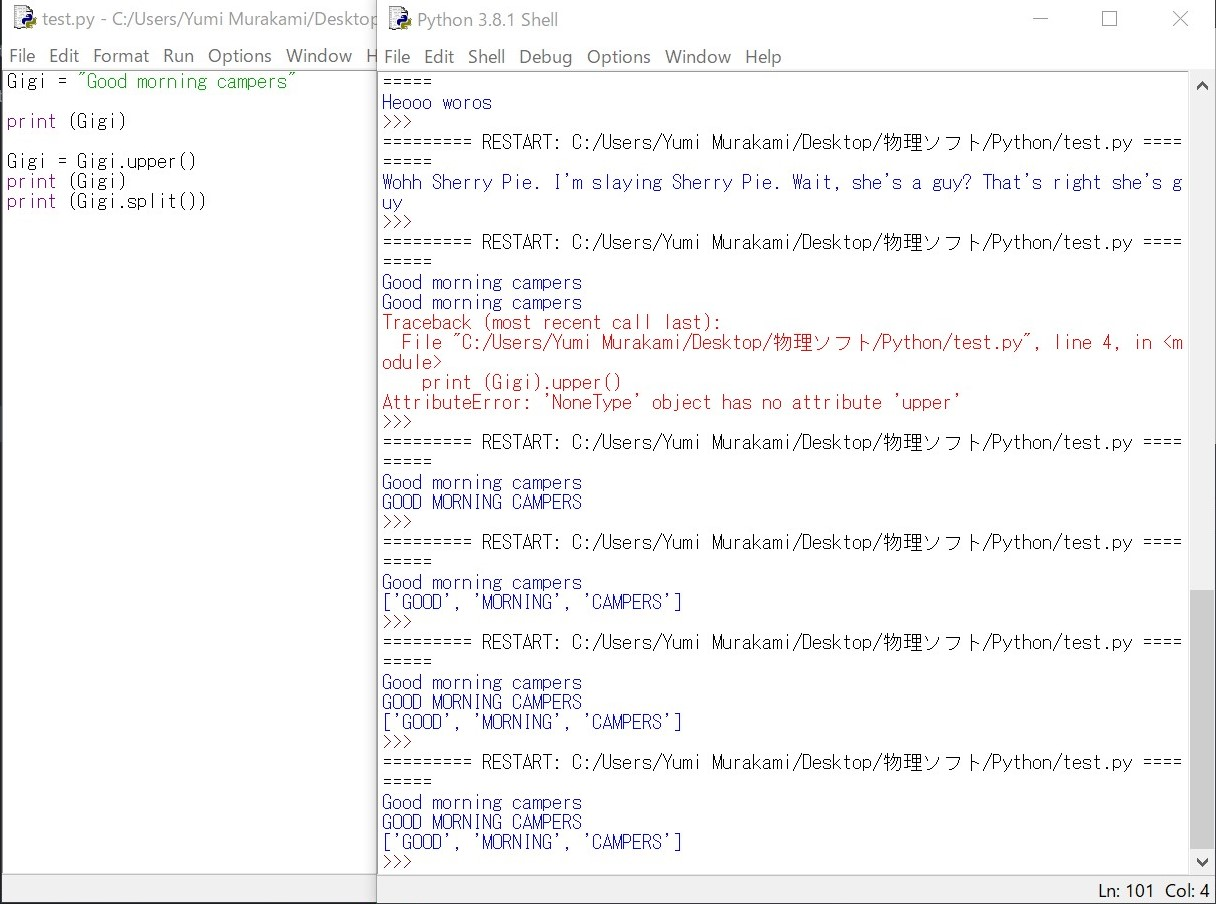
\includegraphics[clip,height=7.0cm]{how_to_use_variables.jpg}
  \caption{how to use variables}
  \label{variables}
 \end{center}
\end{figure}


\section{メソッド}%
メソッド:お尻につけると便利な働きをしてくれるコマンド
\subsection{メソッド入力法}
入力画面:
print ("Hello world".コマンド)

→出力画面に出力\\

メソッドは組み合わせ可能

\subsection{メソッド集}
\begin{table}[htb]
 \begin{tabular}{cc}
  split("A")       & Aを境に分割                        \\
  replace("A","B") & AをBに置き換え                     \\
  upper()          & 小文字を大文字に置き換え           \\
  lower()          & 大文字を小文字に置き換え           \\
  join(変数)       & ばらばらの文字列をつなげる         \\
  find("文字列")   & 特定の文字列が何番目かを教える     \\
  count("文字列")  & 特定の文字列が登場する個数を教える
 \end{tabular}

\end{table}

\subsection{メソッド入力例}
\subsubsection{join}

\begin{figure}[htbp]
 \begin{center}
  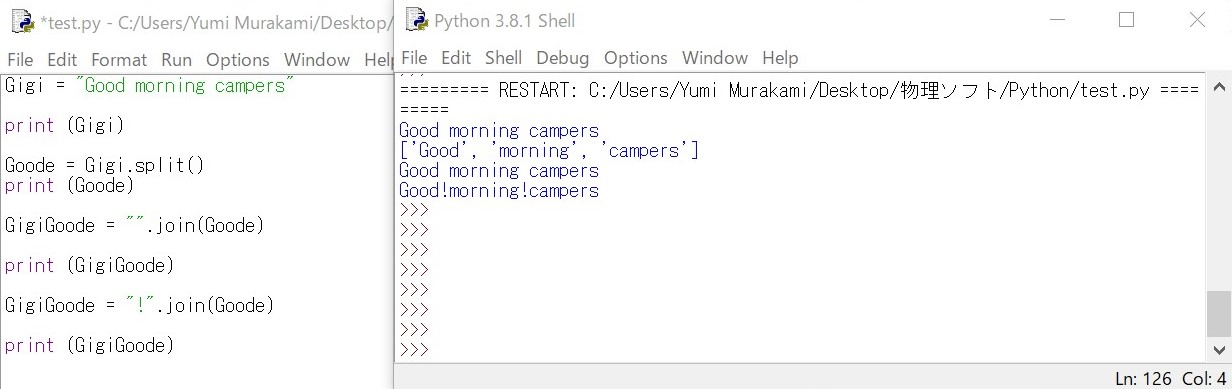
\includegraphics[clip,width=13.0cm]{how_to_use_join.jpg}
  \caption{how to use join}
  \label{join}
 \end{center}
\end{figure}


\end{document}
